\section{Sprint 7 : Déploiement, supervision et DevSecOps}

\subsection{Introduction}

Après les six Sprints fonctionnels, ce dernier Sprint porte sur les conditions dans lesquelles la plateforme est livrée et maintenue en exploitation. Il ne développe aucune fonctionnalité métier nouvelle : il formalise la chaîne d'intégration et de livraison continues, le modèle de déploiement des différents services, la supervision de l'application en production et la démarche DevSecOps appliquée au projet.

Le terme DevSecOps prolonge la logique DevOps en intégrant les contrôles de sécurité directement dans la chaîne d'automatisation, plutôt qu'en fin de cycle. Dans ce projet, cette démarche se traduit par trois exigences : chaque modification doit être vérifiée automatiquement avant d'être livrée ; aucun secret ne doit être exposé côté navigateur ni committé dans le dépôt ; l'application en production doit pouvoir être surveillée, diagnostiquée et restaurée.

La plateforme est composée de plusieurs services aux technologies différentes, ce qui rend l'automatisation indispensable. Une vérification du frontend ne garantit pas celle du backend, et la livraison du service d'analyse des anomalies relève d'un processus distinct. La chaîne mise en place couvre donc le frontend et le backend ; le service d'analyse conserve son propre processus de livraison.

Le chapitre présente les objectifs et le Sprint Backlog, puis la conception de la chaîne d'intégration, du modèle de déploiement et de la sécurité applicative. Il décrit ensuite les fonctionnalités et les configurations réalisées, notamment les contrôles automatiques, les points de santé, les métriques et les alertes, avant de présenter les tests de validation et les limites constatées de la démarche.

\subsection{Objectifs du Sprint}

L'objectif principal de ce Sprint est de rendre la plateforme vérifiable, livrable et observable, afin qu'une modification puisse être contrôlée automatiquement puis mise en production dans des conditions maîtrisées.

Les objectifs spécifiques sont les suivants :

\begin{itemize}
    \item automatiser les contrôles de qualité du frontend et du backend ;
    \item exécuter les tests unitaires, les tests de bout en bout et les tests d'interface à chaque modification ;
    \item mesurer la couverture et soumettre le projet à une quality gate ;
    \item auditer les dépendances et analyser le dépôt à la recherche de vulnérabilités ;
    \item garantir la séparation entre les variables publiques et les secrets serveur ;
    \item sécuriser le backend par des en-têtes HTTP, une validation stricte des entrées, une limitation du débit et des délais d'exécution ;
    \item déclarer les services de production et leurs points de santé ;
    \item ne déclencher le déploiement qu'après la réussite des contrôles ;
    \item vérifier la disponibilité réelle des services après le déploiement ;
    \item exposer des métriques techniques et métier ;
    \item produire des journaux exploitables et remonter les erreurs d'exécution ;
    \item collecter ces métriques et configurer des alertes ;
    \item documenter la procédure de retour arrière et les limites de la démarche.
\end{itemize}

À la fin du Sprint, une modification du dépôt doit être validée ou refusée automatiquement, et la version déployée doit pouvoir être surveillée depuis un tableau de bord.

\subsection{Sprint Backlog}

Le tableau~\ref{tab:sprint7-backlog} recense les tâches planifiées pour ce Sprint.

{\footnotesize
\setlength{\tabcolsep}{4pt}
\begin{longtable}{|p{0.9cm}|>{\raggedright\arraybackslash}p{9.1cm}|>{\raggedright\arraybackslash}p{1.6cm}|>{\raggedright\arraybackslash}p{1.6cm}|}
\caption{Sprint Backlog du Sprint 7}
\label{tab:sprint7-backlog}\\
\hline
\textbf{ID} & \textbf{Tâche} & \textbf{Priorité} & \textbf{Statut} \\
\hline
\endfirsthead

\hline
\textbf{ID} & \textbf{Tâche} & \textbf{Priorité} & \textbf{Statut} \\
\hline
\endhead

S7-01 &
Mettre en place les contrôles d'hygiène du dépôt et la vérification des fichiers de dépendances. &
Moyenne & Réalisé \\
\hline

S7-02 &
Automatiser l'analyse statique, le typage et les tests du frontend avec couverture. &
Haute & Réalisé \\
\hline

S7-03 &
Automatiser les tests d'interface Playwright. &
Haute & Réalisé \\
\hline

S7-04 &
Automatiser les tests du backend, la vérification des index et la compilation. &
Haute & Réalisé \\
\hline

S7-05 &
Exécuter les tests de bout en bout du backend dans la chaîne d'intégration. &
Haute & Réalisé \\
\hline

S7-06 &
Intégrer l'analyse SonarCloud et bloquer la chaîne en cas d'échec de la quality gate. &
Haute & Réalisé \\
\hline

S7-07 &
Auditer les dépendances de production et analyser le dépôt avec Trivy. &
Haute & Réalisé \\
\hline

S7-08 &
Durcir la configuration du backend : en-têtes, validation, limitation du débit et délais. &
Haute & Réalisé \\
\hline

S7-09 &
Séparer les variables publiques des secrets et empêcher leur fuite dans le bundle. &
Haute & Réalisé \\
\hline

S7-10 &
Déclarer les services de production dans une configuration d'infrastructure. &
Haute & Réalisé \\
\hline

S7-11 &
Déclencher le déploiement après intégration continue et protéger l'environnement de production. &
Haute & Réalisé \\
\hline

S7-12 &
Vérifier la disponibilité des services après chaque déploiement. &
Haute & Réalisé \\
\hline

S7-13 &
Exposer les métriques techniques et métier du backend. &
Moyenne & Réalisé \\
\hline

S7-14 &
Mettre en place la collecte Prometheus, le tableau de bord Grafana et les alertes. &
Moyenne & Réalisé \\
\hline

S7-15 &
Documenter le retour arrière, la rotation des secrets et les limites de la démarche. &
Moyenne & Réalisé \\
\hline

S7-16 &
Activer la journalisation structurée et le suivi des erreurs, sous réserve de configuration. &
Moyenne & Réalisé \\
\hline

\end{longtable}}

User Stories associées :

\begin{itemize}
    \item \textbf{US15 :} en tant que responsable du projet, je souhaite automatiser les contrôles de qualité, les tests et le déploiement afin de fiabiliser les livraisons ;
    \item \textbf{US16 :} en tant que responsable du projet, je souhaite superviser les services déployés afin de détecter et de diagnostiquer les incidents.
\end{itemize}

\subsection{Conception du Sprint}

\subsubsection{Vue d'ensemble de la chaîne DevSecOps}

La figure~\ref{fig:architecture-devsecops} situe les composants du projet les uns par rapport aux autres : le poste de développement et le dépôt distant, la chaîne d'intégration continue, les services de production et les outils de supervision.

\begin{figure}[H]
    \centering
    \IfFileExists{figures/architecture-devsecops.png}{%
        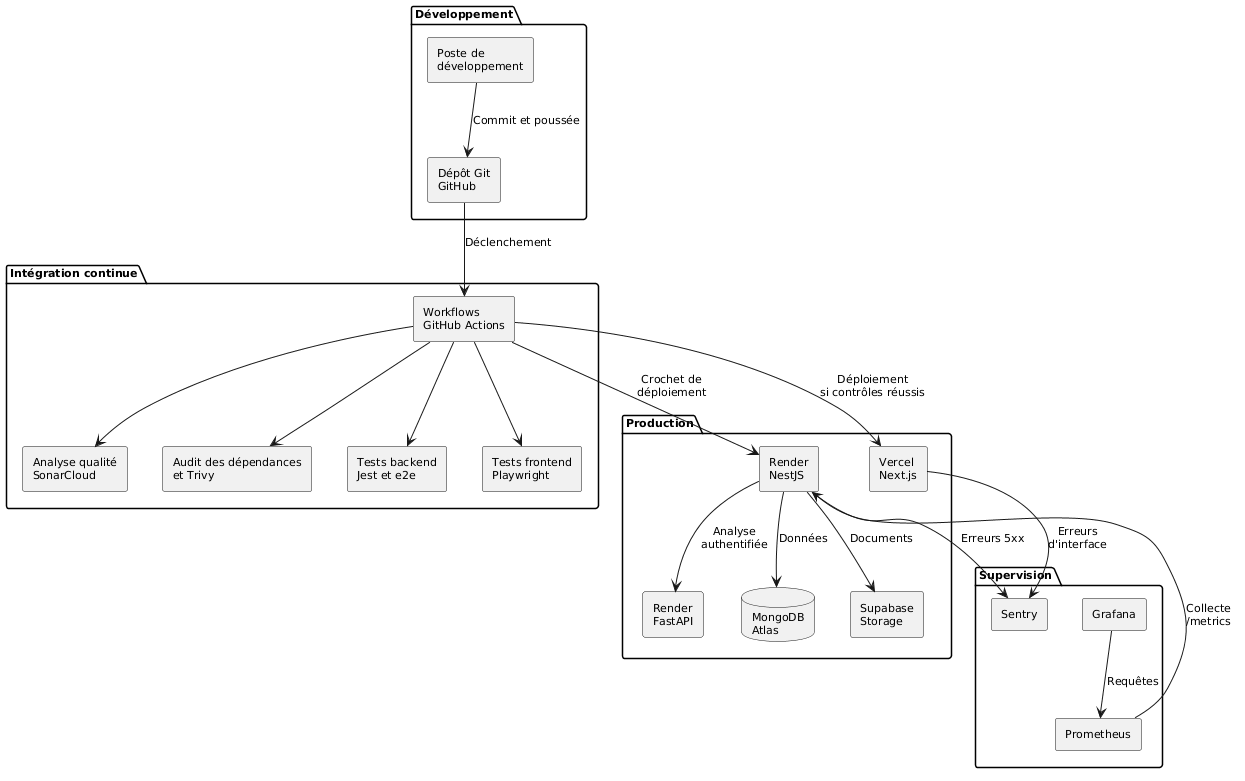
\includegraphics[width=0.78\textwidth,height=0.40\textheight,keepaspectratio]{figures/architecture-devsecops.png}%
    }{%
        \fbox{\parbox[c][7cm][c]{0.92\textwidth}{\centering\itshape Diagramme à insérer\\[2mm]\texttt{figures/architecture-devsecops.png}}}%
    }
    \caption{Architecture DevSecOps de la plateforme}
    \label{fig:architecture-devsecops}
\end{figure}

Cette vue met en évidence deux principes. D'une part, le frontend et le backend ne sont livrés qu'à travers la chaîne d'intégration : aucune de leurs versions ne rejoint la production sans avoir franchi les contrôles. D'autre part, la supervision est un ensemble de consommateurs : Prometheus interroge les métriques du backend, Grafana interroge Prometheus et Sentry reçoit les erreurs signalées par les applications. Aucun de ces outils n'agit sur la plateforme, ce qui limite le risque qu'une supervision défaillante perturbe le service.

Le service d'analyse FastAPI constitue une exception dans ce schéma. Il possède son propre processus de livraison et n'est pas déclenché par la chaîne du dépôt principal, dont il ne partage que le code. Cette séparation est assumée et documentée ; elle implique que ses évolutions doivent être vérifiées manuellement avant leur mise en service.

\subsubsection{Chaîne d'intégration et de livraison}

La chaîne d'automatisation est décrite par deux fichiers de workflow : \texttt{ci-pr.yml} pour l'intégration continue et \texttt{cd-deploy.yml} pour la livraison \cite{github_actions_docs}. Le premier s'exécute sur chaque demande de fusion et sur chaque poussée vers les branches \texttt{main} et \texttt{develop} ; il enchaîne une succession de contrôles indépendants.

Le second n'est pas déclenché directement par le dépôt, mais par l'achèvement du premier : il écoute l'événement de fin d'exécution de la chaîne d'intégration sur la branche \texttt{main} et ne poursuit que si celle-ci s'est terminée avec succès. Une exécution échouée, y compris sur une branche de développement, ne déclenche donc aucun déploiement : la plateforme vérifie la conclusion de la chaîne avant de démarrer la tâche de livraison. Une poussée directe sur \texttt{develop} est ainsi contrôlée sans être livrée.

La figure~\ref{fig:pipeline-cicd} présente cette organisation en quatre couloirs. Le premier regroupe les contrôles d'hygiène du dépôt. Le deuxième réunit les vérifications de qualité du frontend et du backend, y compris les tests d'interface et les tests de bout en bout. Le troisième rassemble les contrôles de sécurité et l'analyse SonarCloud. Le quatrième correspond à la livraison : elle n'est déclenchée que si l'ensemble des contrôles précédents aboutit, puis elle attend la confirmation de disponibilité des services.

\begin{figure}[H]
    \centering
    \IfFileExists{figures/pipeline-cicd.png}{%
        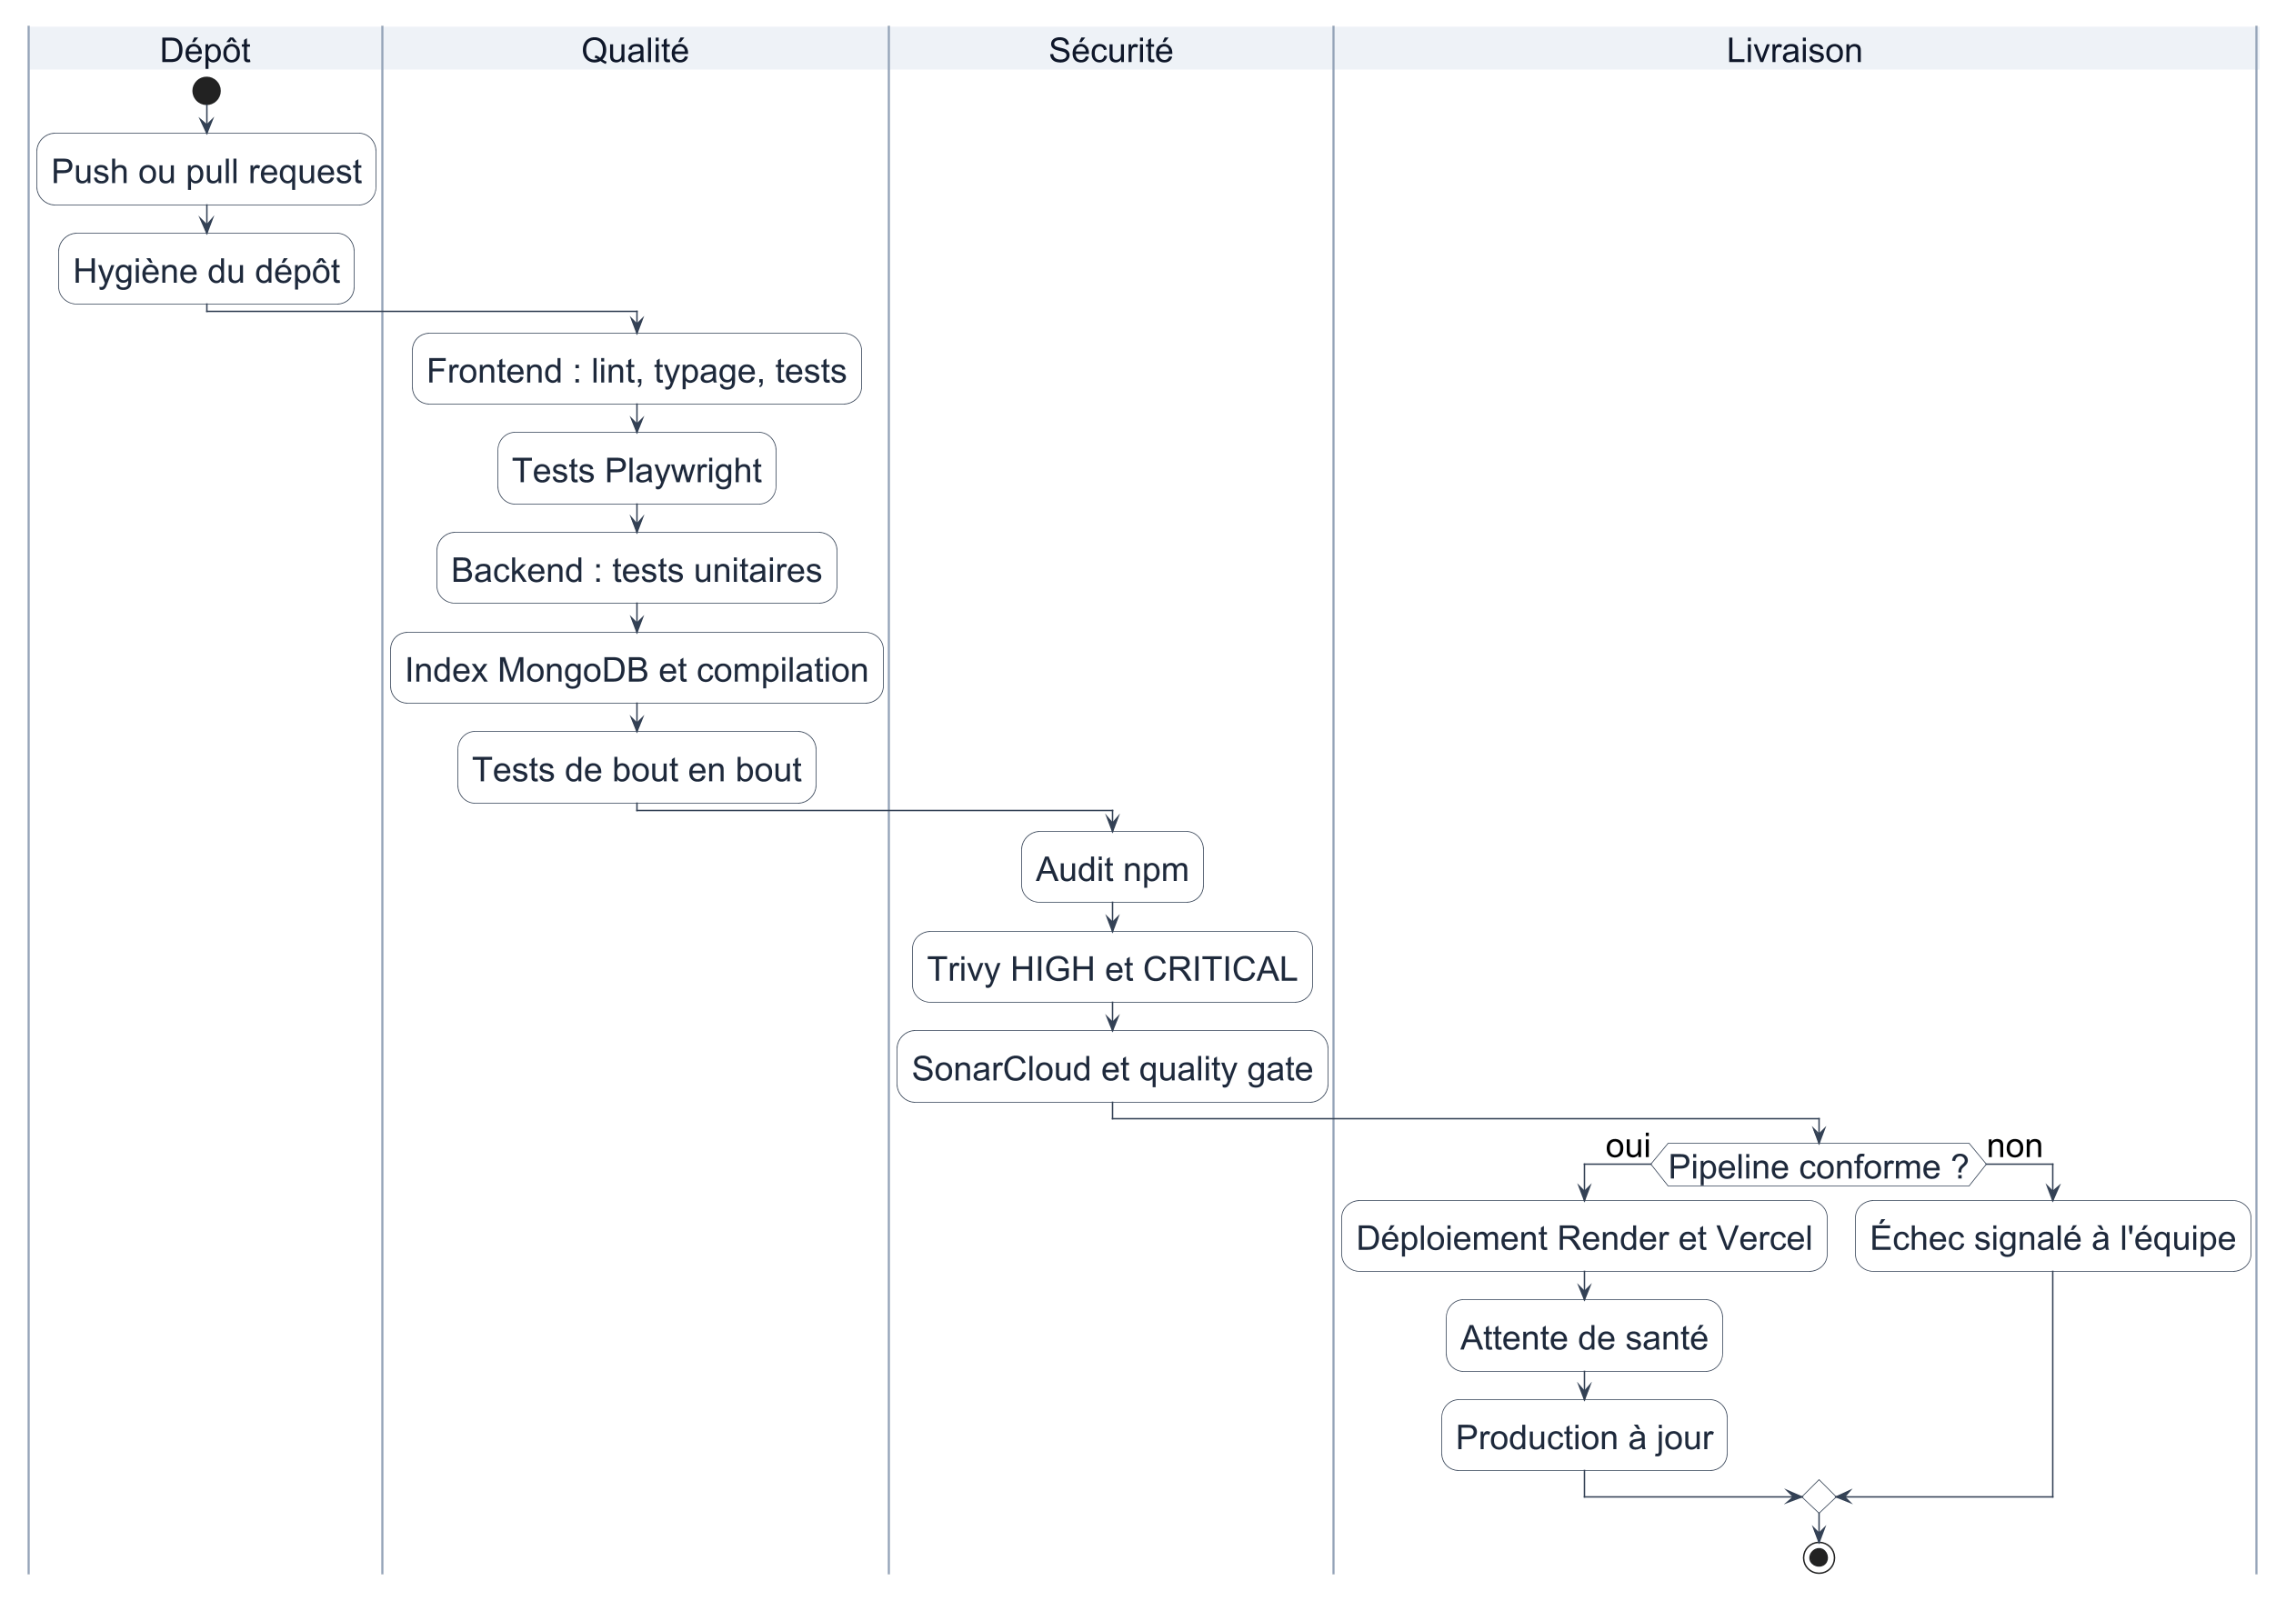
\includegraphics[width=0.92\textwidth,height=0.40\textheight,keepaspectratio]{figures/pipeline-cicd.png}%
    }{%
        \fbox{\parbox[c][7cm][c]{0.92\textwidth}{\centering\itshape Diagramme à insérer\\[2mm]\texttt{figures/pipeline-cicd.png}}}%
    }
    \caption{Chaîne d'intégration et de livraison continues}
    \label{fig:pipeline-cicd}
\end{figure}

Cette organisation suit les recommandations du cadre SSDF du NIST, qui prévoit la vérification automatique du code, des dépendances et des configurations avant la livraison \cite{nist_ssdf}. Les contrôles sont répartis en tâches parallèles lorsque cela est possible, afin de réduire la durée du retour d'information. Une exécution en cours est annulée lorsqu'une nouvelle poussée intervient sur la même branche, ce qui évite d'accumuler des résultats devenus obsolètes. Les droits du jeton d'exécution sont limités à la lecture du contenu du dépôt pour les tâches de vérification.

Deux points de contrôle conditionnent la suite de la chaîne. L'analyse SonarCloud attend explicitement le verdict de la quality gate et échoue si celui-ci n'est pas favorable. Les analyses de sécurité, fondées sur l'audit des dépendances et sur Trivy \cite{trivy_docs}, échouent également lorsque des vulnérabilités de niveau élevé ou critique sont détectées. En revanche, le rapport détaillé de ces analyses est transmis à l'onglet de sécurité du dépôt même lorsque la chaîne échoue, afin de conserver la trace des anomalies.

L'exécution présentée ci-dessous regroupe les contrôles d'hygiène du dépôt, de qualité du frontend et du backend, les tests de bout en bout, l'analyse SonarCloud et les contrôles de sécurité.

\begin{figure}[H]
    \centering
    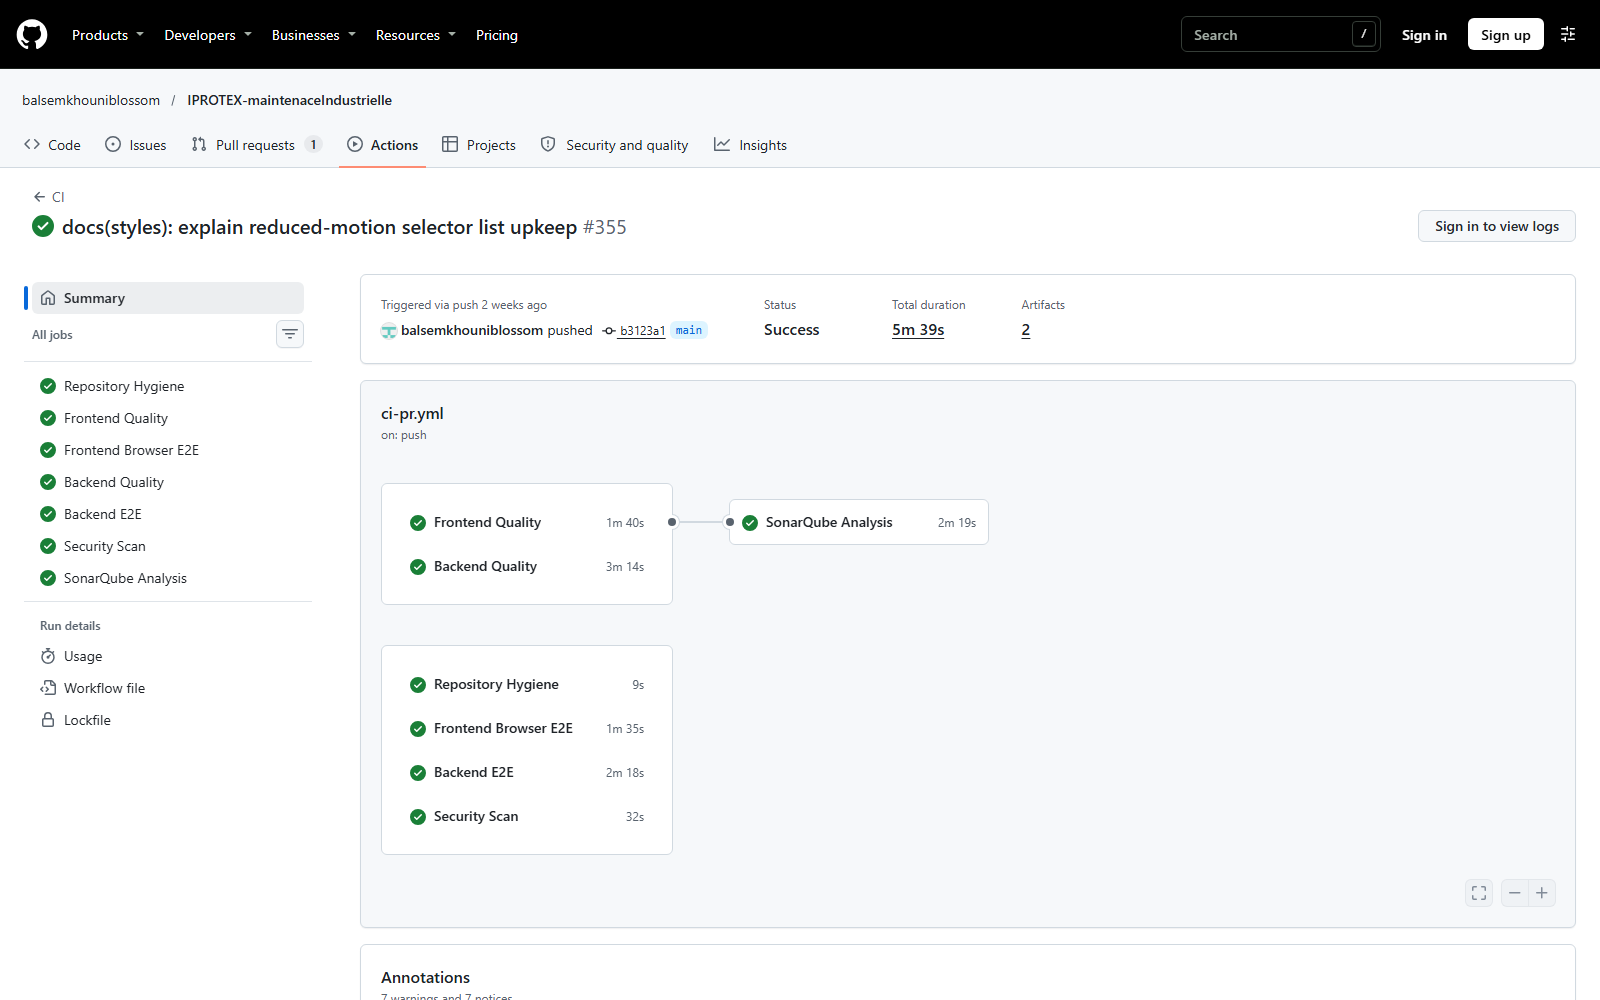
\includegraphics[width=0.92\textwidth,height=0.72\textheight,keepaspectratio]{figures/captures/sprint7-ci-pipeline.png}
    \caption{Exécution des contrôles de la chaîne d'intégration continue}
    \label{fig:sprint7-ci-pipeline}
\end{figure}

\subsubsection{Architecture de déploiement}

Les composants ne sont pas hébergés sur une même infrastructure. Le frontend est déployé sur une plateforme spécialisée dans les applications Next.js, tandis que le backend, le service d'analyse et les services de supervision sont hébergés sur une plateforme de services web. La figure~\ref{fig:architecture-deploiement} présente cette répartition et les flux entre composants.

\begin{figure}[H]
    \centering
    \IfFileExists{figures/architecture-deploiement.png}{%
        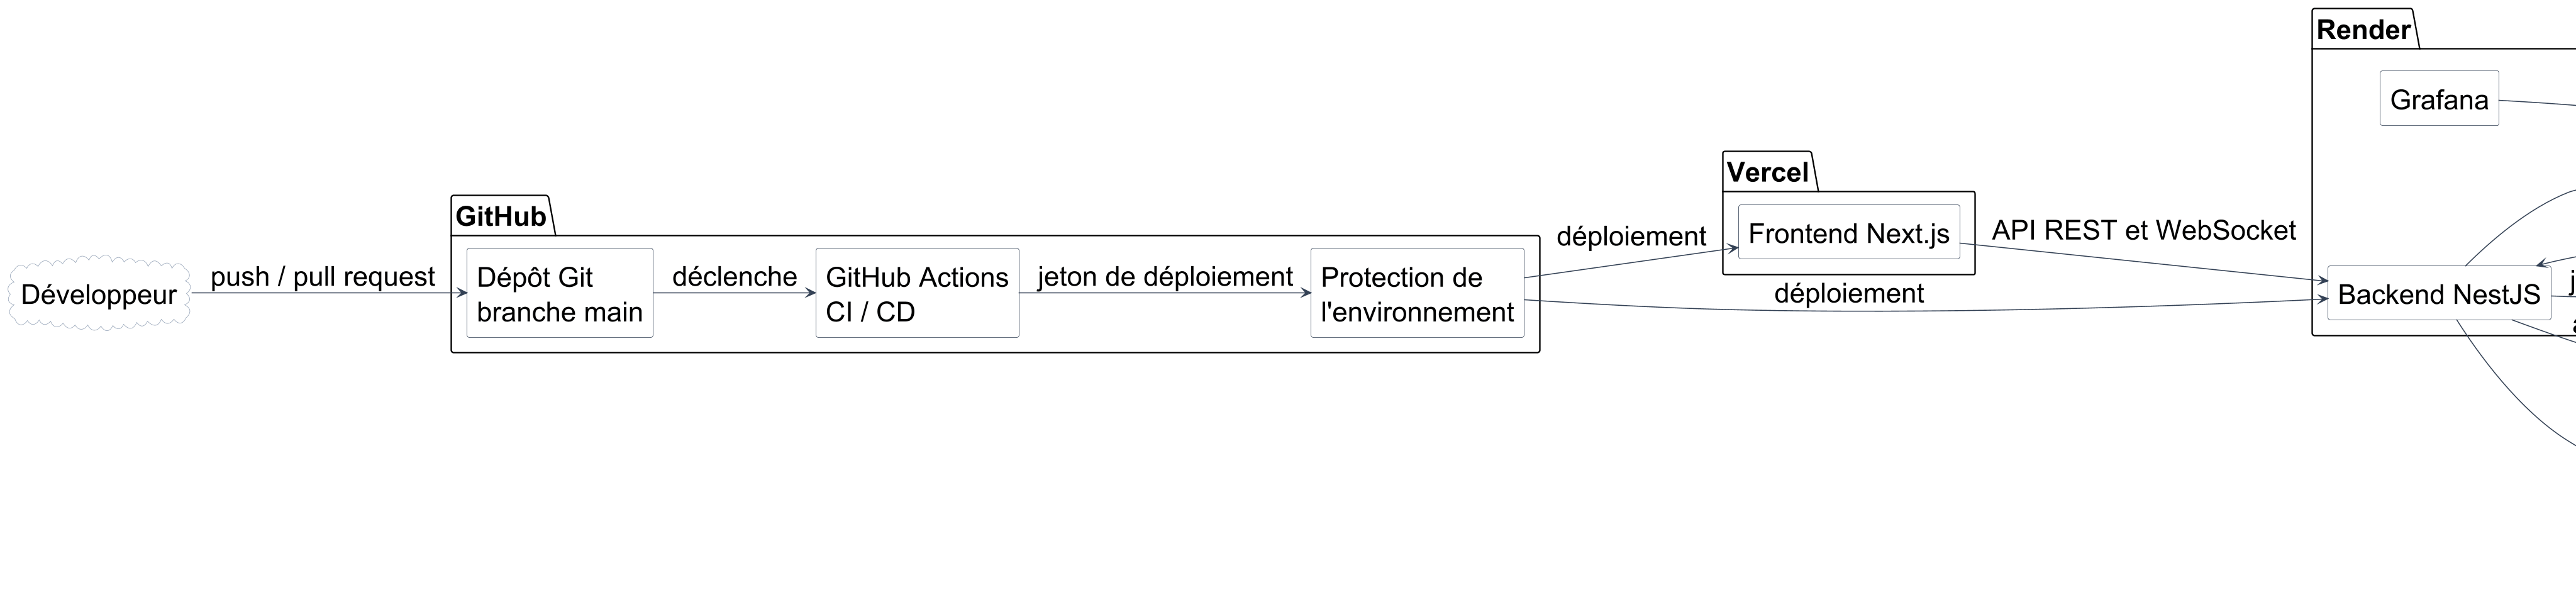
\includegraphics[width=\textwidth,height=0.26\textheight,keepaspectratio]{figures/architecture-deploiement.png}%
    }{%
        \fbox{\parbox[c][7cm][c]{0.92\textwidth}{\centering\itshape Diagramme à insérer\\[2mm]\texttt{figures/architecture-deploiement.png}}}%
    }
    \caption{Architecture de déploiement de la plateforme}
    \label{fig:architecture-deploiement}
\end{figure}

Le navigateur ne dialogue qu'avec le frontend, qui appelle ensuite l'API du backend en REST et par WebSocket. Le backend accède à la base MongoDB Atlas et au stockage de documents, et il appelle le service d'analyse avec un jeton de service distinct des identifiants utilisateurs. Ce service est isolé du reste du système : il n'a pas accès à la base applicative et se limite à recevoir des mesures et à renvoyer un score.

Les services de supervision occupent une position particulière. Prometheus interroge l'endpoint de métriques du backend à intervalle régulier, et Grafana interroge Prometheus pour alimenter ses tableaux de bord. Cette chaîne est unidirectionnelle : la supervision lit les métriques, elle n'agit pas sur l'application.

La configuration d'infrastructure décrit ces services de manière reproductible. Elle précise pour chacun la commande de construction, la commande de démarrage, le chemin de vérification de santé et les variables d'environnement attendues. Les valeurs sensibles sont déclarées sans contenu et renseignées dans l'interface de la plateforme, ce qui évite qu'un identifiant soit présent dans le dépôt. La livraison automatique est désactivée sur ces services : un déploiement ne se produit que lorsqu'il est déclenché par la chaîne de livraison.

\subsubsection{Séquence de livraison}

La figure~\ref{fig:sequence-deploiement} présente le déroulement d'une mise en production. Après la fusion d'une modification sur la branche principale, la chaîne exécute les contrôles, puis déclenche le déploiement du backend et celui du frontend.

\begin{figure}[H]
    \centering
    \IfFileExists{figures/sequence-deploiement.png}{%
        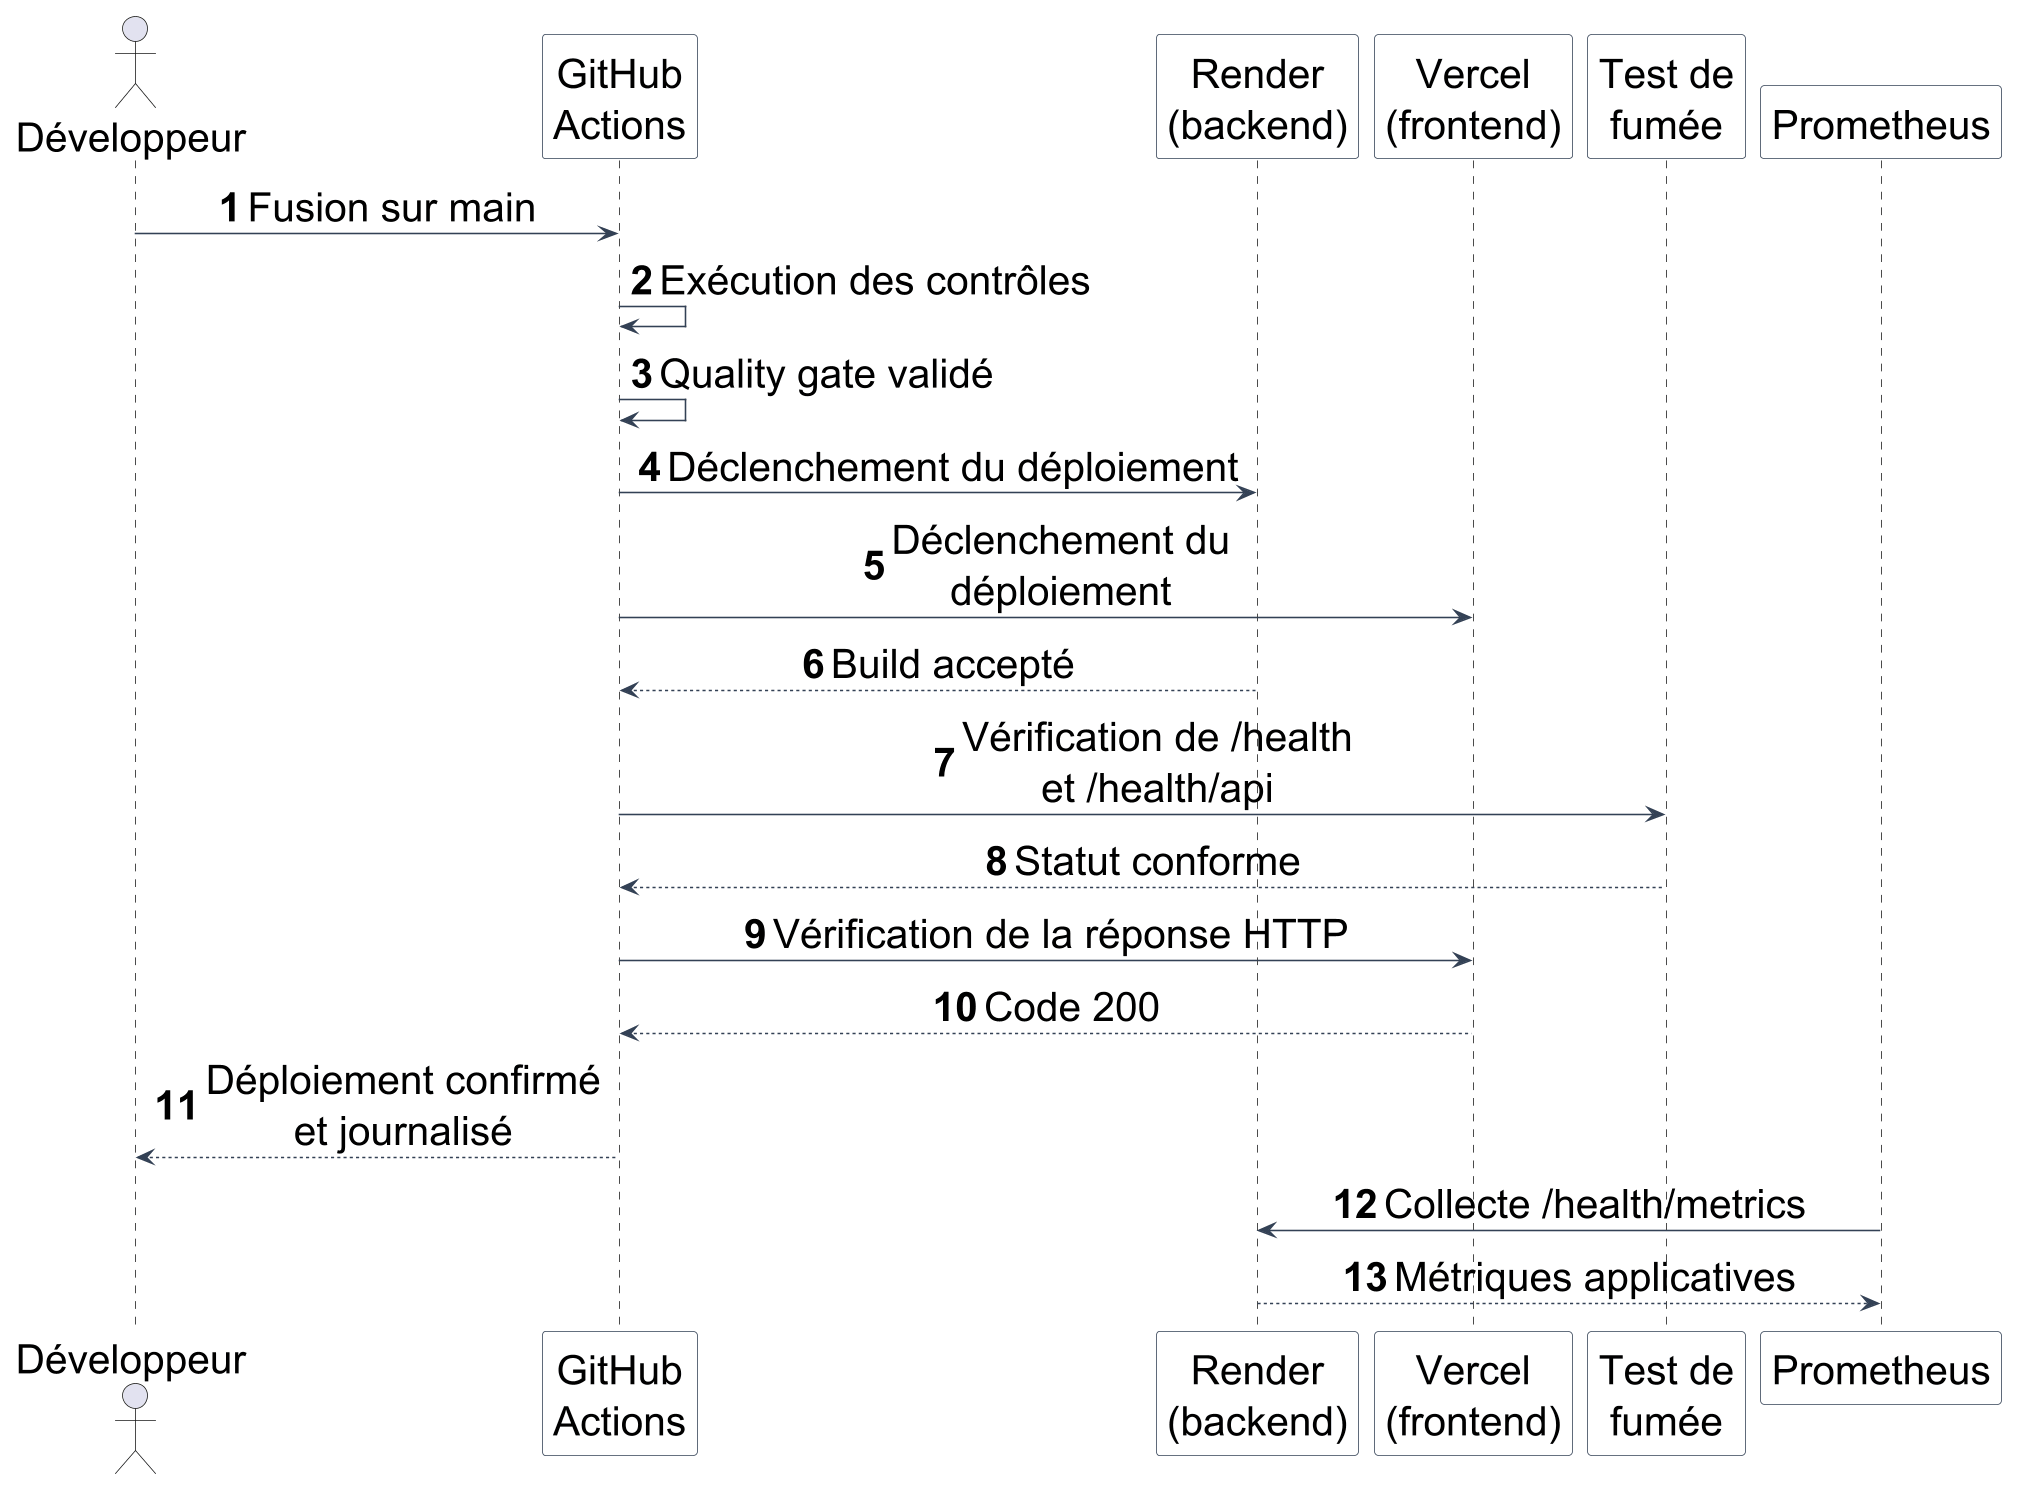
\includegraphics[width=0.84\textwidth,height=0.26\textheight,keepaspectratio]{figures/sequence-deploiement.png}%
    }{%
        \fbox{\parbox[c][7cm][c]{0.92\textwidth}{\centering\itshape Diagramme à insérer\\[2mm]\texttt{figures/sequence-deploiement.png}}}%
    }
    \caption{Diagramme de séquence du déploiement en production}
    \label{fig:sequence-deploiement}
\end{figure}

Un déclencheur de déploiement ne confirme que l'acceptation de la demande par la plateforme, et non la disponibilité de la nouvelle version. C'est pourquoi la chaîne interroge ensuite le service jusqu'à vingt fois, à quinze secondes d'intervalle. Le backend est considéré comme disponible si les points de santé répondent avec le statut attendu ; le frontend est considéré comme disponible s'il répond avec un code 200. Si le délai est dépassé, la chaîne échoue et le motif est consigné dans le résumé d'exécution. Une version acceptée mais incapable de démarrer est ainsi détectée par l'automatisation plutôt que par un utilisateur.

\subsubsection{Sécurité applicative}

La sécurité de la plateforme repose sur plusieurs barrières indépendantes, dont l'organisation suit les recommandations de l'ASVS de l'OWASP \cite{owasp_asvs}. Au niveau du serveur, les en-têtes HTTP appliquent une politique restrictive : le backend ne sert que du JSON et quelques fichiers statiques, aucune page HTML, aucun script et aucun cadre. La validation des requêtes refuse par défaut tout champ non déclaré, ce qui réduit la surface d'attaque des interfaces de programmation.

La limitation du débit est configurée globalement et selon le type de client, avec un quota distinct pour les équipements connectés. Un délai maximal d'exécution empêche qu'une requête bloque indéfiniment un traitement. La taille des corps de requête est bornée explicitement, de même que celle des messages transmis par les équipements.

Au niveau de la configuration, les variables sont validées au démarrage : une valeur manquante ou incohérente interrompt le lancement du service plutôt que de produire un fonctionnement dégradé silencieux. Le service d'analyse applique le même principe, avec une vérification de disponibilité qui échoue si l'artefact du modèle ne peut pas être chargé.

La séparation des secrets constitue une exigence structurante. Les variables préfixées \texttt{NEXT\_PUBLIC} sont seules exposées au navigateur ; les identifiants de base de données, les clés de signature, les clés de stockage et les jetons de service restent côté serveur. Un test automatisé contrôle le code source et la configuration du frontend afin de détecter l'introduction d'un nom de secret serveur ou d'une référence non sécurisée dans le bundle.

\subsection{Réalisation}

\subsubsection{Organisation du dépôt et des versions}

Le code source est conservé dans un dépôt Git hébergé sur GitHub, qui regroupe les trois applications, la configuration d'infrastructure, les scripts d'exploitation, les diagrammes et la documentation. Ce regroupement permet de versionner ensemble le code et les fichiers qui le décrivent, ce qui évite qu'une modification de configuration soit appliquée sans être tracée.

La branche principale, \texttt{main}, reflète l'état livrable. Les évolutions sont développées sur des branches dédiées, intégrées par demande de fusion après vérification des contrôles. Les messages de commit suivent une convention de préfixe qui indique la nature du changement — correction, évolution, documentation, tâche d'infrastructure —, ce qui rend l'historique lisible et permet de filtrer les modifications par catégorie. Le journal prend ainsi la forme \texttt{fix(styles)}, \texttt{docs(...)} ou \texttt{chore: ...} selon le cas.

Une règle de contribution accompagne ce fonctionnement : toute modification du comportement, de l'installation ou des procédures doit être répercutée dans la documentation correspondante, et les diagrammes doivent être mis à jour lorsque les services, les dépendances ou les frontières du système changent. Cette exigence a été appliquée dans ce rapport : les diagrammes du Sprint 7 décrivent l'état réel des workflows, et non une intention.

L'historique du dépôt contient néanmoins des branches de sauvegarde antérieures à une opération de nettoyage. Leur présence rappelle que la maîtrise de l'historique fait partie de l'hygiène du dépôt : les fichiers sensibles supprimés d'une branche restent accessibles dans les commits antérieurs, ce qui est précisément le cas de l'incident décrit dans les limites de ce chapitre.

\subsubsection{Intégration continue}

La chaîne d'intégration regroupe sept tâches. La première vérifie l'hygiène du dépôt : elle refuse la présence d'artefacts d'exécution suivis et contrôle la cohérence des fichiers de verrouillage des dépendances. La deuxième exécute l'analyse statique, le typage, les tests unitaires avec couverture et la compilation du frontend. La troisième exécute les tests d'interface du navigateur. La quatrième réalise les mêmes vérifications sur le backend, auxquelles s'ajoutent la création effective des index MongoDB sur une base de test et la compilation de production. La cinquième exécute les tests de bout en bout du backend sur une base isolée. La sixième réalise l'analyse SonarCloud à partir des rapports de couverture produits par les tâches précédentes. La septième effectue les contrôles de sécurité.

Les tests unitaires s'appuient sur une base MongoDB éphémère fournie par le service d'intégration, ce qui garantit des résultats reproductibles sans accès à la base de production. La quality gate et la couverture sont gérées par SonarCloud \cite{sonarcloud_docs}. La couverture est produite au format standard et les chemins de sources sont vérifiés avant transmission à SonarCloud, afin d'éviter qu'un rapport mal formé ne soit accepté silencieusement.

Le tableau~\ref{tab:controles-ci} synthétise ces tâches, les vérifications qu'elles portent et l'effet d'un échec sur la livraison.

{\footnotesize
\setlength{\tabcolsep}{4pt}
\begin{longtable}{|>{\raggedright\arraybackslash}p{3.4cm}|>{\raggedright\arraybackslash}p{7.2cm}|>{\raggedright\arraybackslash}p{3.8cm}|}
\caption{Synthèse des contrôles automatisés}
\label{tab:controles-ci}\\
\hline
\textbf{Tâche} & \textbf{Vérifications} & \textbf{Effet en cas d'échec} \\
\hline
\endfirsthead

\hline
\textbf{Tâche} & \textbf{Vérifications} & \textbf{Effet en cas d'échec} \\
\hline
\endhead

Hygiène du dépôt &
Artefacts d'exécution suivis, cohérence des fichiers de verrouillage &
Chaîne arrêtée \\
\hline

Qualité frontend &
Analyse statique, typage, tests avec couverture, compilation &
Chaîne arrêtée \\
\hline

Tests d'interface &
Scénarios de navigateur Playwright &
Chaîne arrêtée \\
\hline

Qualité backend &
Analyse statique, tests avec couverture, création des index, compilation &
Chaîne arrêtée \\
\hline

Tests de bout en bout &
Scénarios d'API sur une base MongoDB isolée &
Chaîne arrêtée \\
\hline

Analyse SonarCloud &
Couverture globale et quality gate &
Chaîne arrêtée après l'analyse \\
\hline

Contrôles de sécurité &
Audit npm des dépendances de production, analyse Trivy &
Chaîne arrêtée, rapport transmis \\
\hline

\end{longtable}}

Le dépôt compte 202 fichiers de tests unitaires côté backend, 26 fichiers de tests de bout en bout et 44 fichiers de tests côté frontend, auxquels s'ajoutent les scénarios d'interface Playwright. Cette volumétrie explique la durée de la chaîne et justifie la parallélisation des tâches.

\subsubsection{Contrôles de sécurité}

L'audit des dépendances est exécuté séparément sur le frontend et sur le backend, en ne considérant que les dépendances de production. Le seuil retenu bloque la chaîne à partir du niveau modéré, ce qui est plus strict que le niveau élevé souvent utilisé par défaut. L'analyse du système de fichiers recherche les vulnérabilités de niveau élevé et critique dans le code et les configurations, en excluant les répertoires de dépendances et de construction. Le rapport produit est transmis à l'onglet de sécurité du dépôt.

Les actions tierces utilisées dans la chaîne de sécurité et d'analyse sont référencées par empreinte de commit plutôt que par étiquette de version. Une étiquette peut être déplacée par son éditeur ; une empreinte identifie un contenu immuable. Cette pratique limite le risque qu'une action compromise soit exécutée avec les secrets du dépôt.

\subsubsection{Déploiement et variables d'environnement}

La livraison est protégée par un environnement dédié, ce qui permet de restreindre les secrets utilisés lors d'un déploiement en production. Deux mécanismes de déclenchement sont prévus pour le backend : un déclencheur de déploiement et un appel à l'interface de programmation de la plateforme d'hébergement. Le second sert de solution de repli si le premier échoue, et la chaîne n'est déclarée réussie que si l'un des deux aboutit.

Les variables sont organisées selon leur destinataire. Le frontend ne reçoit que l'adresse de l'API et les paramètres publics. Le backend reçoit les identifiants de base de données, les clés de signature des jetons, les paramètres d'envoi de courriel, les clés de stockage et le jeton du service d'analyse. Prometheus reçoit un jeton dédié, distinct de toute session utilisateur, afin que la collecte ne dépende pas d'un compte dont l'accès expire.

Le service d'analyse reçoit un jeton de service partagé avec le backend, comparé de manière résistante aux attaques temporelles, ainsi que des limites de taille de requête et de nombre de lignes par lot. Ces limites protègent le service d'une saturation par un appel volumineux.

\subsubsection{Supervision et métriques}

Le backend expose un endpoint de santé et un endpoint de métriques. Le premier agrège l'état de l'API, de la base de données et du transport de courriel ; il renvoie un état dégradé lorsque le transport de courriel est indisponible, sans pour autant signaler une panne de l'application. Des points de santé spécifiques permettent d'isoler la vivacité du processus, l'état de l'API, celui de la base et celui du courriel.

L'endpoint de métriques renvoie un format textuel standard, lisible par Prometheus \cite{prometheus_docs}. Il expose des métriques techniques, comme le nombre de requêtes par route et par statut, la durée des requêtes ou l'état du processus, et des métriques métier, comme le nombre d'ordres de travail ouverts, les heures d'arrêt machine, les interventions terminées et les pièces en stock faible.

L'accès à cet endpoint est protégé. Il accepte soit un jeton d'administration, soit le jeton dédié configuré pour la collecte. Prometheus utilise le second, ce qui évite de dépendre d'une session utilisateur et de ses renouvellements.

Grafana \cite{grafana_docs} est provisionné avec la source de données Prometheus et un tableau de bord dédié. Ce tableau de bord présente l'état du backend, le volume de requêtes, le taux d'erreur, le temps de réponse, les routes les plus sollicitées et les indicateurs métier. Les alertes configurées couvrent trois situations : l'absence de collecte pendant plus de deux minutes, un taux d'erreurs serveur supérieur à 0,05 par seconde sur cinq minutes et une latence moyenne supérieure à une seconde sur dix minutes. Ces indicateurs relèvent de la pratique de fiabilité des services, qui privilégie l'observation de la disponibilité, des erreurs et de la latence plutôt que la seule vérification fonctionnelle \cite{sre_book}.

\subsubsection{Journaux et suivi des erreurs}

Les métriques indiquent qu'un service se dégrade ; elles ne disent pas quelle requête a échoué ni pour quel utilisateur. Le diagnostic repose donc sur les journaux et sur le suivi des erreurs d'exécution.

Chaque requête reçoit un identifiant de corrélation. Il provient de l'en-tête \texttt{x-request-id} lorsqu'il est fourni et respecte un format attendu, sinon il est généré. Cet identifiant est renvoyé dans la réponse et repris dans la ligne de journal correspondante, ce qui permet de relier une erreur signalée par un utilisateur à son traitement côté serveur.

Le format des journaux dépend de l'environnement. En développement, les lignes restent lisibles sous forme de texte. En production, le paramètre \texttt{LOG\_FORMAT} est fixé à \texttt{json} : chaque requête produit un objet d'une seule ligne, contenant l'horodatage, l'identifiant de corrélation, la méthode, le chemin, le statut et la durée de traitement. Ce format se prête à l'analyse automatique par les outils de la plateforme d'hébergement, qui collecte la sortie standard des services. Il n'existe pas, à ce stade, d'agrégateur de journaux distinct : la conservation et la recherche s'appuient sur l'interface de la plateforme.

Le suivi des erreurs est assuré par Sentry \cite{sentry_docs}, activé uniquement lorsqu'une clé de collecte est fournie. Le backend charge cette instrumentation avant tout autre module, afin que l'interception soit effective dès le démarrage. Le filtre global d'exceptions transmet au service les seules erreurs serveur inattendues, accompagnées de l'identifiant de corrélation et du contexte de la requête. Les erreurs de client, qui relèvent d'une requête mal formée et non d'un défaut de l'application, sont journalisées sans être remontées, afin de ne pas saturer la file d'incidents.

Côté frontend, l'instrumentation est répartie entre le serveur, l'exécution en périphérie et le navigateur. Le SDK n'est chargé dans le navigateur que si la clé publique correspondante est définie, ce qui évite d'alourdir le bundle lorsque le suivi est désactivé. Les erreurs d'affichage capturées par les frontières d'erreur de l'application sont centralisées en un point unique, qui associe à chaque événement la frontière concernée, l'empreinte de l'erreur et la pile des composants. Les secrets du fournisseur restent côté serveur ; seule la clé publique est exposée.

En l'absence de clé configurée, l'ensemble de ces appels reste sans effet et n'interrompt pas le fonctionnement de la plateforme. Le suivi des erreurs est donc une capacité disponible, dont l'activation relève de l'exploitation.

\subsubsection{Retour arrière et exploitation}

Les deux plateformes d'hébergement conservent l'historique des déploiements. Un retour arrière réactive une version antérieure : sans reconstruction pour le frontend, et sans modification des variables d'environnement pour le backend. Cette opération ne restaure pas la base de données : une incompatibilité de schéma doit être traitée par une correction en avant, après vérification des index.

La procédure de sauvegarde couvre la base, les fichiers et le code, avec une vérification de l'intégrité des archives. Ces archives ne sont jamais versionnées, car un export de base peut contenir des empreintes de mots de passe et des jetons de rafraîchissement.

\subsection{Tests et validation}

Le tableau~\ref{tab:tests-sprint7} présente les scénarios de test retenus pour ce Sprint. Ces scénarios portent sur la chaîne elle-même et sur le comportement des services déployés, et non sur une fonctionnalité métier.

{\footnotesize
\setlength{\tabcolsep}{4pt}
\begin{longtable}{|p{0.9cm}|>{\raggedright\arraybackslash}p{7cm}|>{\raggedright\arraybackslash}p{4.7cm}|}
\caption{Scénarios de test du Sprint 7}
\label{tab:tests-sprint7}\\
\hline
\textbf{ID} & \textbf{Scénario} & \textbf{Résultat attendu} \\
\hline
\endfirsthead

\hline
\textbf{ID} & \textbf{Scénario} & \textbf{Résultat attendu} \\
\hline
\endhead

T7-01 &
Présence d'un artefact d'exécution suivi par Git &
Tâche d'hygiène en échec \\
\hline

T7-02 &
Erreur de typage dans le frontend &
Compilation refusée et chaîne en échec \\
\hline

T7-03 &
Échec d'un scénario Playwright &
Tâche d'interface en échec \\
\hline

T7-04 &
Test backend en échec &
Tâche de qualité backend en échec \\
\hline

T7-05 &
Index MongoDB non créables &
Tâche d'index en échec \\
\hline

T7-06 &
Échec d'un test de bout en bout &
Tâche de bout en bout en échec \\
\hline

T7-07 &
Quality gate SonarCloud non satisfaite &
Chaîne arrêtée après l'analyse \\
\hline

T7-08 &
Vulnérabilité modérée dans une dépendance de production &
Audit en échec \\
\hline

T7-09 &
Vulnérabilité critique détectée par Trivy &
Analyse en échec et rapport transmis \\
\hline

T7-10 &
Tentative de fusion avec une chaîne en échec &
Déploiement non déclenché \\
\hline

T7-11 &
Backend déployé mais incapable de démarrer &
Attente de santé en échec après vingt tentatives \\
\hline

T7-12 &
Frontend répondant avec un code autre que 200 &
Attente de disponibilité en échec \\
\hline

T7-13 &
Appel des métriques sans jeton valide &
Accès refusé \\
\hline

T7-14 &
Collecte Prometheus avec le jeton dédié &
Métriques techniques et métier reçues \\
\hline

T7-15 &
Backend injoignable pendant plus de deux minutes &
Alerte critique déclenchée \\
\hline

T7-16 &
Latence moyenne supérieure à une seconde pendant dix minutes &
Alerte de latence déclenchée \\
\hline

T7-17 &
Variable obligatoire absente au démarrage &
Service arrêté avec message explicite \\
\hline

T7-18 &
Référence à un secret serveur dans le frontend &
Test de non-exposition en échec \\
\hline

T7-19 &
Requête traitée avec \texttt{LOG\_FORMAT=json} &
Ligne JSON unique avec horodatage, identifiant et statut \\
\hline

T7-20 &
Erreur serveur inattendue avec une clé Sentry définie &
Événement transmis avec l'identifiant de corrélation \\
\hline

T7-21 &
Erreur serveur inattendue sans clé Sentry &
Traitement poursuivi, aucun envoi \\
\hline

\end{longtable}}

Les tests confirment que la chaîne refuse une modification défaillante avant la livraison et qu'un déploiement accepté mais non fonctionnel est détecté par l'attente de disponibilité. Ils confirment également que les métriques ne sont accessibles qu'avec un jeton valide et que les alertes se déclenchent sur les seuils configurés.

\subsection{Limites de la démarche}

Plusieurs limites doivent être signalées. La chaîne ne comporte pas d'environnement intermédiaire : une fusion sur la branche principale conduit directement en production. Aucun analyseur de secrets n'y est exécuté, l'automatisation des mises à jour de dépendances n'est pas configurée et les images de conteneurs ne sont pas analysées, alors que des fichiers de construction existent. Le service d'analyse des anomalies a ses propres tests d'API, mais il n'est pas exécuté par la chaîne, qui couvre le frontend et le backend : une régression de ce service ne serait pas détectée.

Le suivi des erreurs n'est par ailleurs pas encore exploité : aucun projet de collecte n'est associé à la plateforme, si bien que l'instrumentation reste inactive en production. Les journaux sont consultés depuis la plateforme d'hébergement, sans agrégateur ni recherche centralisée.

Enfin, un incident de sécurité est documenté et non résolu : un export de base contenant des empreintes de mots de passe et de jetons de rafraîchissement a été versionné et reste accessible dans l'historique du dépôt distant. La rotation des identifiants et l'invalidation des sessions sont prioritaires. Ce constat illustre l'écart entre des contrôles automatiques et une posture de sécurité vérifiée.

\subsection{Revue du Sprint et conclusion}

Lors de la revue, une modification du dépôt a été suivie depuis la demande de fusion jusqu'à sa mise en production : contrôles, quality gate, déploiement et vérification de disponibilité. Le parcours reprend les scénarios du tableau~\ref{tab:tests-sprint7}. Une modification invalide est arrêtée par la tâche concernée avant toute livraison, tandis qu'une fusion conforme traverse les sept tâches, franchit la quality gate et déclenche le déploiement, suivi de l'attente de disponibilité. L'exploitation a été présentée à partir du tableau de bord Grafana, des seuils d'alerte et de l'accès protégé aux métriques.

La durée de la chaîne a été discutée. La volumétrie des tests, avec plus de deux cents fichiers côté backend, explique un temps de retour de plusieurs minutes. La parallélisation des tâches et l'annulation des exécutions devenues obsolètes ont été présentées comme les deux leviers retenus pour contenir ce délai sans réduire la couverture.

La portée de la supervision a également été précisée. Les métriques et les alertes portent sur le backend : ni le frontend, ni le service d'analyse ne sont instrumentés, si bien qu'une dégradation de l'interface ou une indisponibilité du modèle ne serait pas détectée par les tableaux de bord. Leur disponibilité n'est vérifiée qu'à l'occasion d'un déploiement : le frontend par le contrôle du code HTTP, le service d'analyse par la sonde de disponibilité que la plateforme d'hébergement applique lors de ses propres déploiements. Aucune sonde périodique ne les surveille ensuite. Cette asymétrie tient aux priorités du Sprint, qui a privilégié l'API, point d'entrée unique des données métier.

Les principaux résultats sont les suivants :

\begin{itemize}[nosep,leftmargin=1.2em]
    \item chaîne d'intégration couvrant frontend, backend, tests de bout en bout et quality gate ;
    \item contrôles de sécurité par audit des dépendances et analyse du dépôt ;
    \item déploiement conditionné aux contrôles et vérifié après livraison ;
    \item supervision par métriques protégées, tableau de bord et alertes.
\end{itemize}

La rétrospective a souligné l'écart entre la disponibilité des outils et la maturité de la démarche : les contrôles automatiques sont largement en place, mais l'absence d'environnement de recette, de détection de secrets et de nettoyage de l'historique limite encore la garantie apportée. Les priorités sont la remédiation de l'incident documenté, la mise en place d'un environnement intermédiaire, puis la détection de secrets et l'automatisation des mises à jour.

Ce Sprint clôt la réalisation fonctionnelle et technique de la plateforme ; la conclusion générale revient sur les résultats, les difficultés rencontrées et les perspectives du projet.
